\input{"C:/Users/spileggi/Google Drive/STAT 330/Lectures/SlideStyle.tex"}



\title[Lecture 9]{Data cleaning and new variable creation, formalized}
\author[Pileggi]{Shannon Pileggi}

\institute[STAT 330]{STAT 330}

\date{}


\begin{document}

\begin{frame}
\titlepage
\end{frame}

\begin{frame}
\frametitle{OUTLINE\qquad\qquad\qquad} \tableofcontents[hideallsubsections]
\end{frame}



%===========================================================================================================================
\section[Overview]{Overview}
%===========================================================================================================================
\subsection{}

\begin{frame}
\ft{Steps to data cleaning/new variable creation}
\hspace*{0.3cm}
\begin{itemize}
\item[Step 1:] \textbf{Get to know your data.}
\begin{enumerate}[a.]
\item Identify existing values and/or unusual values
\item Identify if missing values are present
\item Identify how many observations had the unusual values
\item Identify which observations had the unusual values
\end{enumerate}
\item[]
\item[Step 2:] \textbf{Create clean new variables with desired result.}
\begin{enumerate}
\item[] \emph{Over-writing existing variable values could be problematic down the line}
\end{enumerate}
\item[]
\item[Step 3:] \textbf{Verify that coding was done correctly.}
\item[]
\end{itemize}
\end{frame}

\begin{frame}
\ft{What's wrong with \texttt{PROC PRINT} for verification?}
\begin{itemize}
\item Viewing your data with \texttt{PROC PRINT}, or otherwise like in the data table viewer, is prone to human error.  Especially with large data sets, it would be very time consuming to visually inspect \emph{all} the data to verify correctness.
\item Too much \texttt{PROC PRINT} eats SAS's memory!  (Think printing thousands of observations, multiple times...) SAS will dramatically slow down, and maybe even crash on you.
\item If you get caught where you have used too much \texttt{PROC PRINT} and SAS is slow, try:
\begin{itemize}
\item the special submit \texttt{F9}
\item close SAS and open it again
\end{itemize}
\end{itemize}
\end{frame}

\begin{frame}
\ft{Limiting \texttt{PROC PRINT}}
You can use \texttt{PROC PRINT} to get a quick glance at your data, but limit the observations printed.
\vskip15pt
\fbox{\texttt{obs = }} \\
\vskip3pt
specifies the \emph{last} observation that SAS processes in a data set.
\vskip15pt
\fbox{\texttt{PROC PRINT DATA = mydata (obs=10) ; RUN ;}}\\
\vskip3pt
prints the first 10 observations
\vskip15pt
\fbox{\texttt{PROC PRINT DATA = mydata (firstobs=5 obs=10) ; RUN ;}}\\
\vskip3pt
prints observations 5 through 10
\end{frame}

\begin{frame}
\fto
\begin{clicker}{For each of the following questions, identify the scenario as: (1) categorical to categorical, (2) quantitative to quantitative, or (3) quantitative to categorical.}
\begin{itemize}
\footnotesize{
\item[\underline{\hspace{0.2in}}] Lab 4 Q6: Create a new variable called \texttt{GPA\_clean} that is a copy of the GPA variable.  Re-code the unusual values missing.
\item[\underline{\hspace{0.2in}}] Lab 4 Q8: Create a new variable called \texttt{prev\_stats} which has a value of \texttt{yes} if students have previous experience with statistics (\texttt{Q03a = 0}) and a value of \texttt{no} if the student does not have previous experience with statistics (\texttt{Q03a = 1}).
\item[\underline{\hspace{0.2in}}] Lab 4 Q11: Create a new variable called \texttt{class} that classifies students as ``lower'' class (first years and second years) and ``upper'' class (third years, fourth years, etc.).
\item[\underline{\hspace{0.2in}}] Lab 4 Q13: Use the \texttt{GPA\_clean} variable to create a new variable called \texttt{honors} that classifies students according to their current GPA; students who do not yet achieve honors should be classified as ``none''.}
\end{itemize}
\end{clicker}
\end{frame}

%===========================================================================================================================
\section[Categorical to Categorical]{Categorical to Categorical}
%===========================================================================================================================
\subsection{}
\begin{frame}
\tableofcontents[currentsection, hideallsubsections]
\end{frame}

\begin{frame}[fragile]
\ft{Step 1: Get to know your data.}
\framesubtitle{\underline{Lab 4 Q11:} Create a new variable called \texttt{class} that classifies students as ``lower'' class (first years and second years) and ``upper'' class (third years, fourth years, etc.).}
\begin{enumerate}[a.]
\item Identify existing values and/or unusual values
\item Identify if missing values are present
\item Identify how many observations had the unusual values
\item Identify which observations had the unusual values
\end{enumerate}
\vskip10pt
\bmp{0.50\textwidth}
\footnotesize
\begin{code}{.0}
PROC FREQ DATA = survey ;
   TABLES Q02 ;
RUN ;
\end{code}
\emp
\bmp{0.02\textwidth} \hspace{1in} \emp
\bmp{0.5\textwidth}
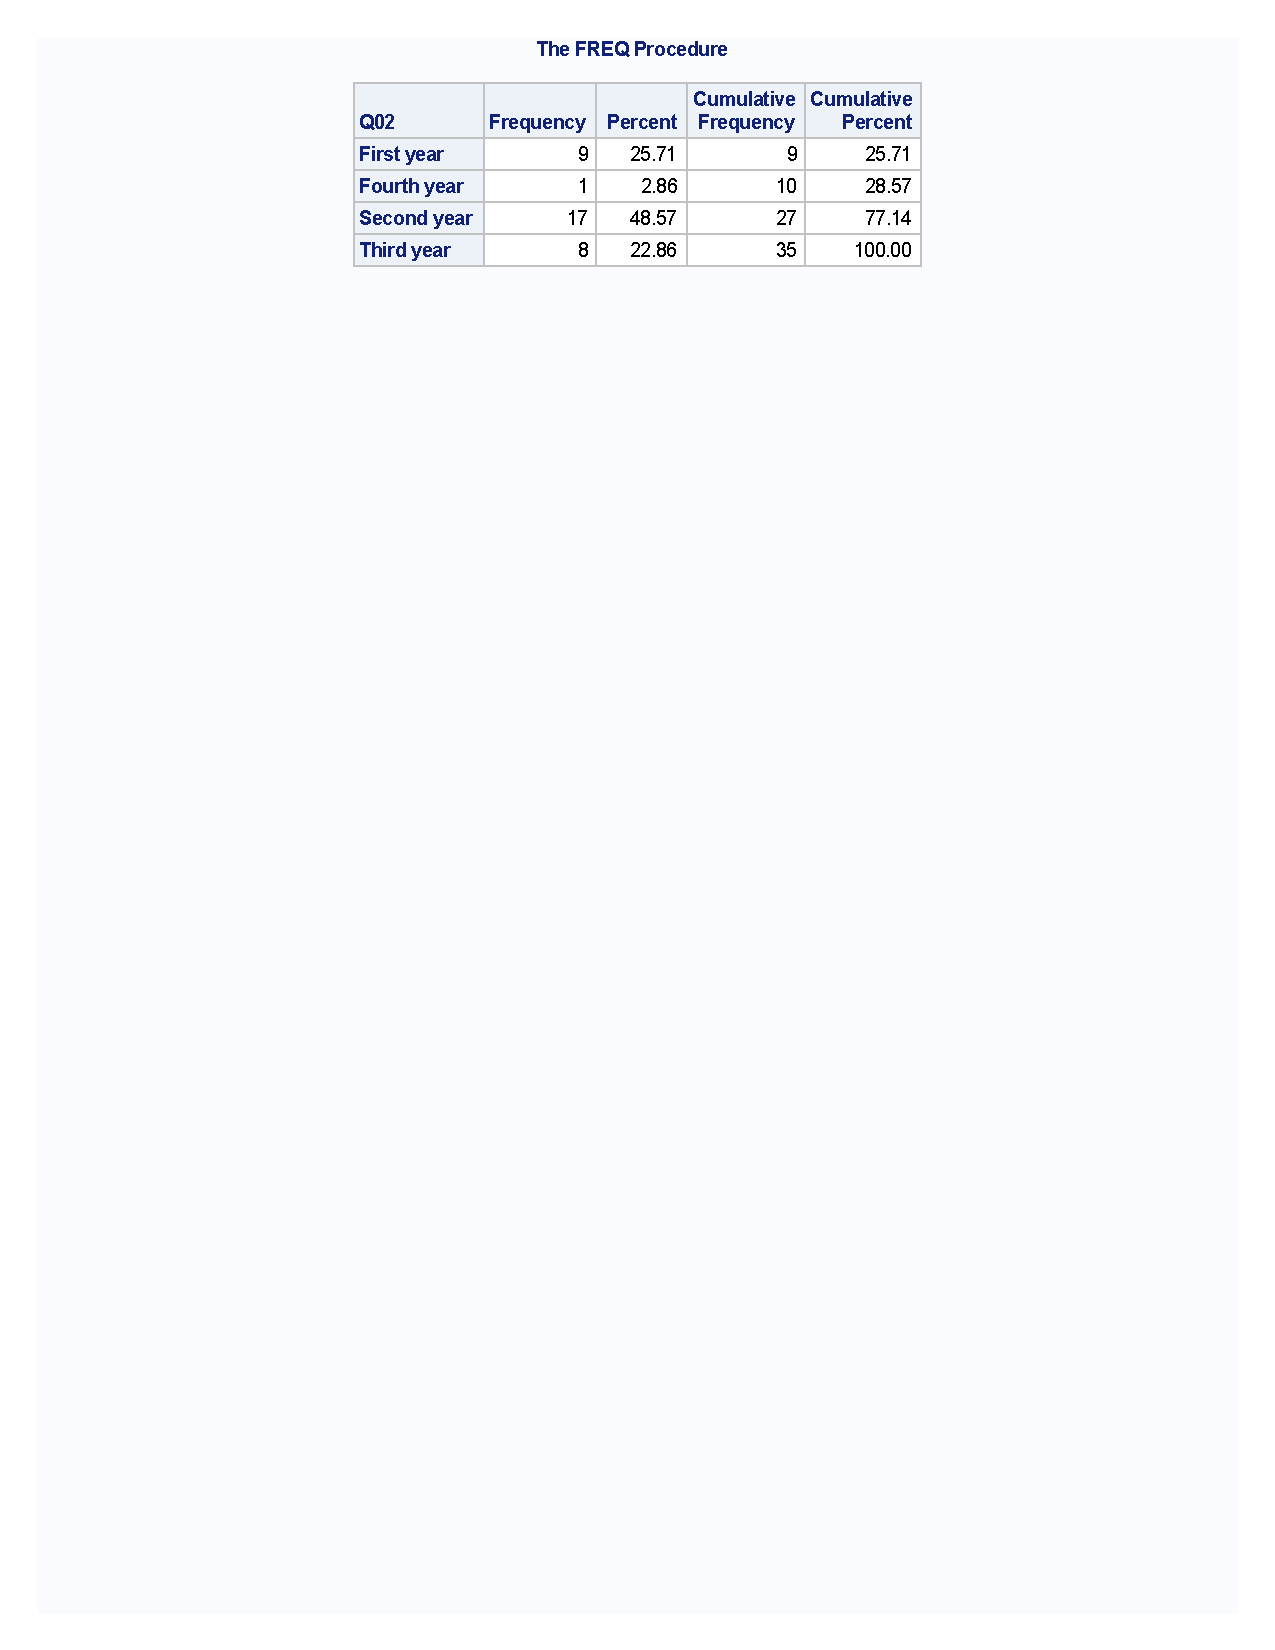
\includegraphics[trim=5cm 22cm 5cm 0.5cm,clip,width=1.0\textwidth]{L9_ccstep1.pdf}
\emp
\end{frame}


\begin{frame}[fragile]
\ft{Step 2: Create clean new variables with desired result.}
\framesubtitle{\underline{Lab 4 Q11:} Create a new variable called \texttt{class} that classifies students as ``lower'' class (first years and second years) and ``upper'' class (third years, fourth years, etc.).}
\bmp{1.02\textwidth}
\footnotesize
\begin{code}{.0}
IF Q02 IN ("First year","Second year") THEN class  = "lower" ;
ELSE class = "upper" ;
\end{code}
\emp
\end{frame}

\begin{frame}[fragile]
\ft{Step 3: Verify that coding was done correctly.}
\framesubtitle{\underline{Lab 4 Q11:} Create a new variable called \texttt{class} that classifies students as ``lower'' class (first years and second years) and ``upper'' class (third years, fourth years, etc.).}
\bmp{0.5\textwidth}
\footnotesize
\begin{code}{.0}
PROC FREQ DATA = survey ;
   TABLES class * Q02 ;
RUN ;
\end{code}
\emp
\bmp{0.02\textwidth} \hspace{1in} \emp
\bmp{0.5\textwidth}
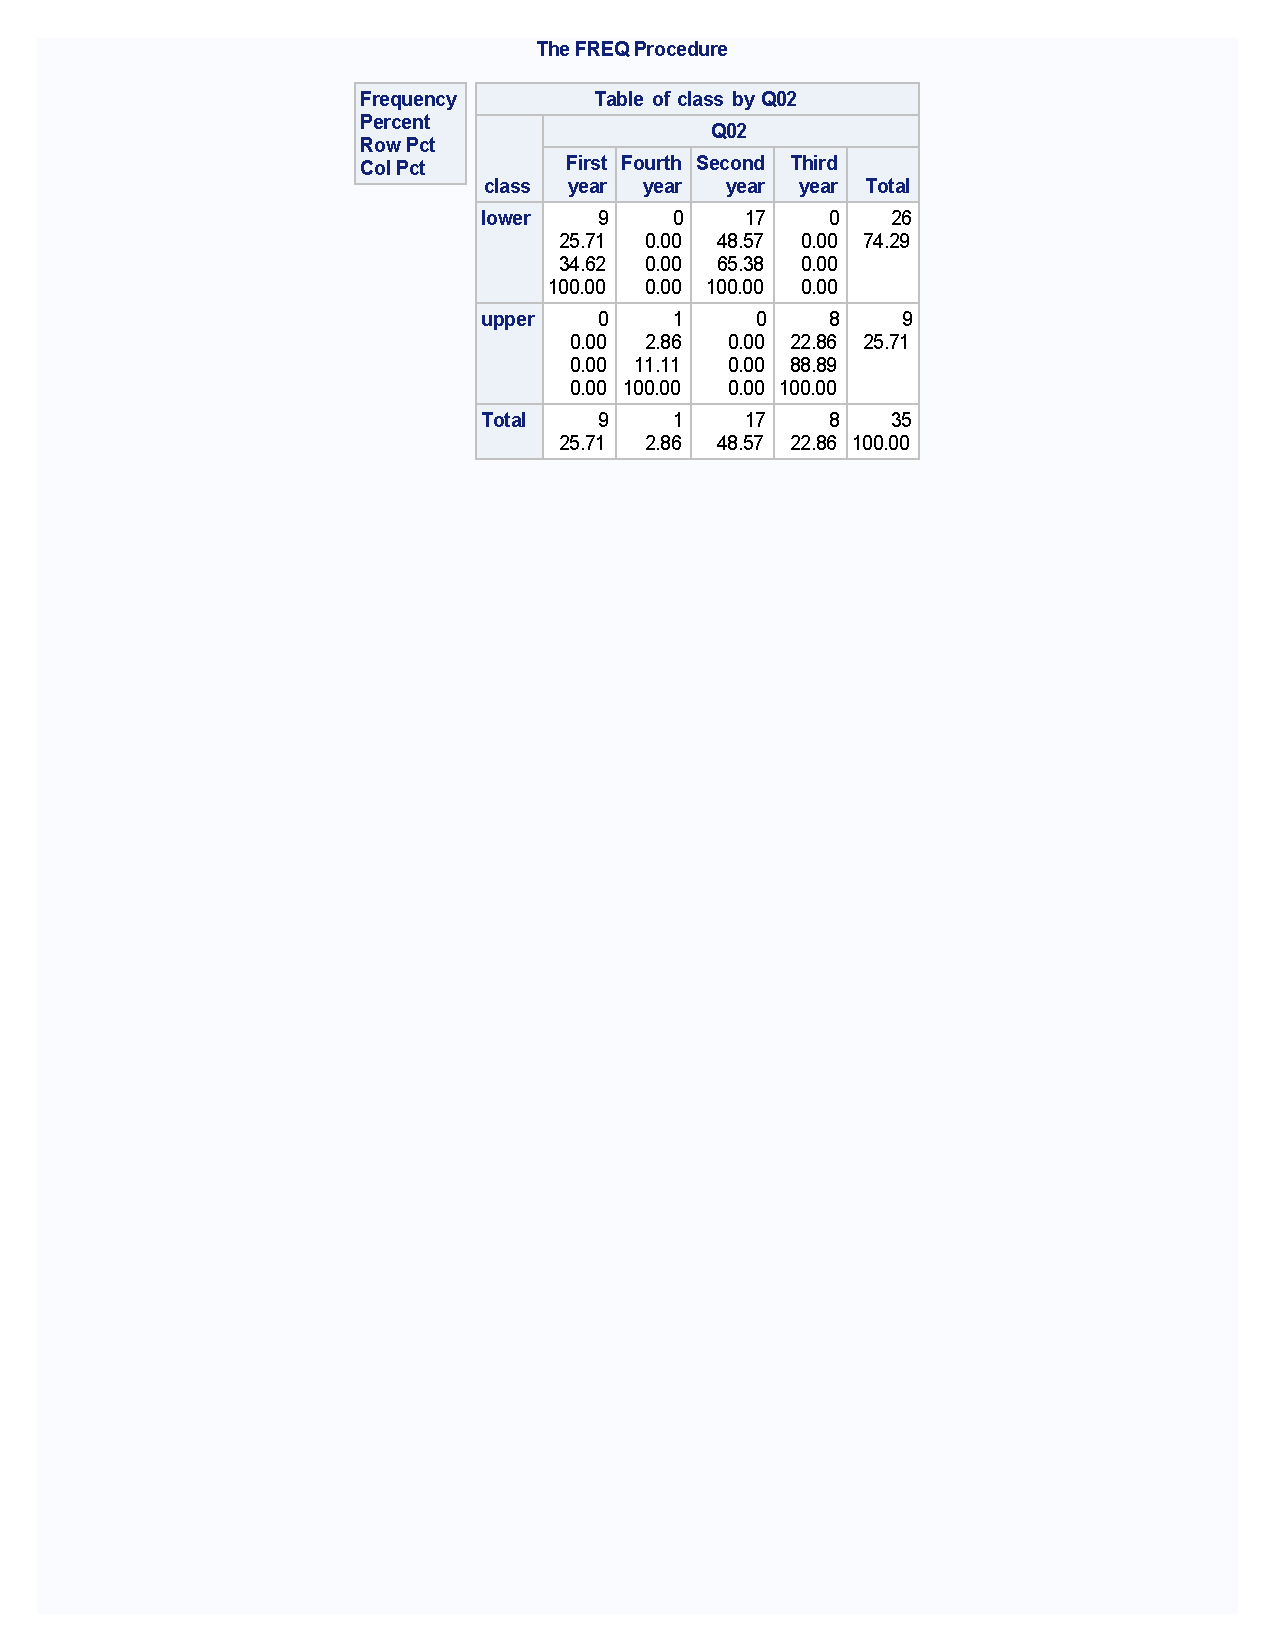
\includegraphics[trim=5cm 20cm 5cm 0.5cm,clip,width=1.0\textwidth]{L9_ccstep3a.pdf}
\emp
\end{frame}

\begin{frame}[fragile]
\ft{Step 3: Verify that coding was done correctly, better.}
\framesubtitle{\underline{Lab 4 Q11:} Create a new variable called \texttt{class} that classifies students as ``lower'' class (first years and second years) and ``upper'' class (third years, fourth years, etc.).}
\begin{itemize}
\item[Step 3:] \textbf{Verify that coding was done correctly.}
\end{itemize}
\vskip10pt
\bmp{0.5\textwidth}
\footnotesize
\begin{code}{.0}
PROC FREQ DATA =  survey ;
   TABLES class * Q02
   / LIST MISSING ;
RUN ;
\end{code}
\emp
\bmp{0.02\textwidth} \hspace{1in} \emp
\bmp{0.5\textwidth}
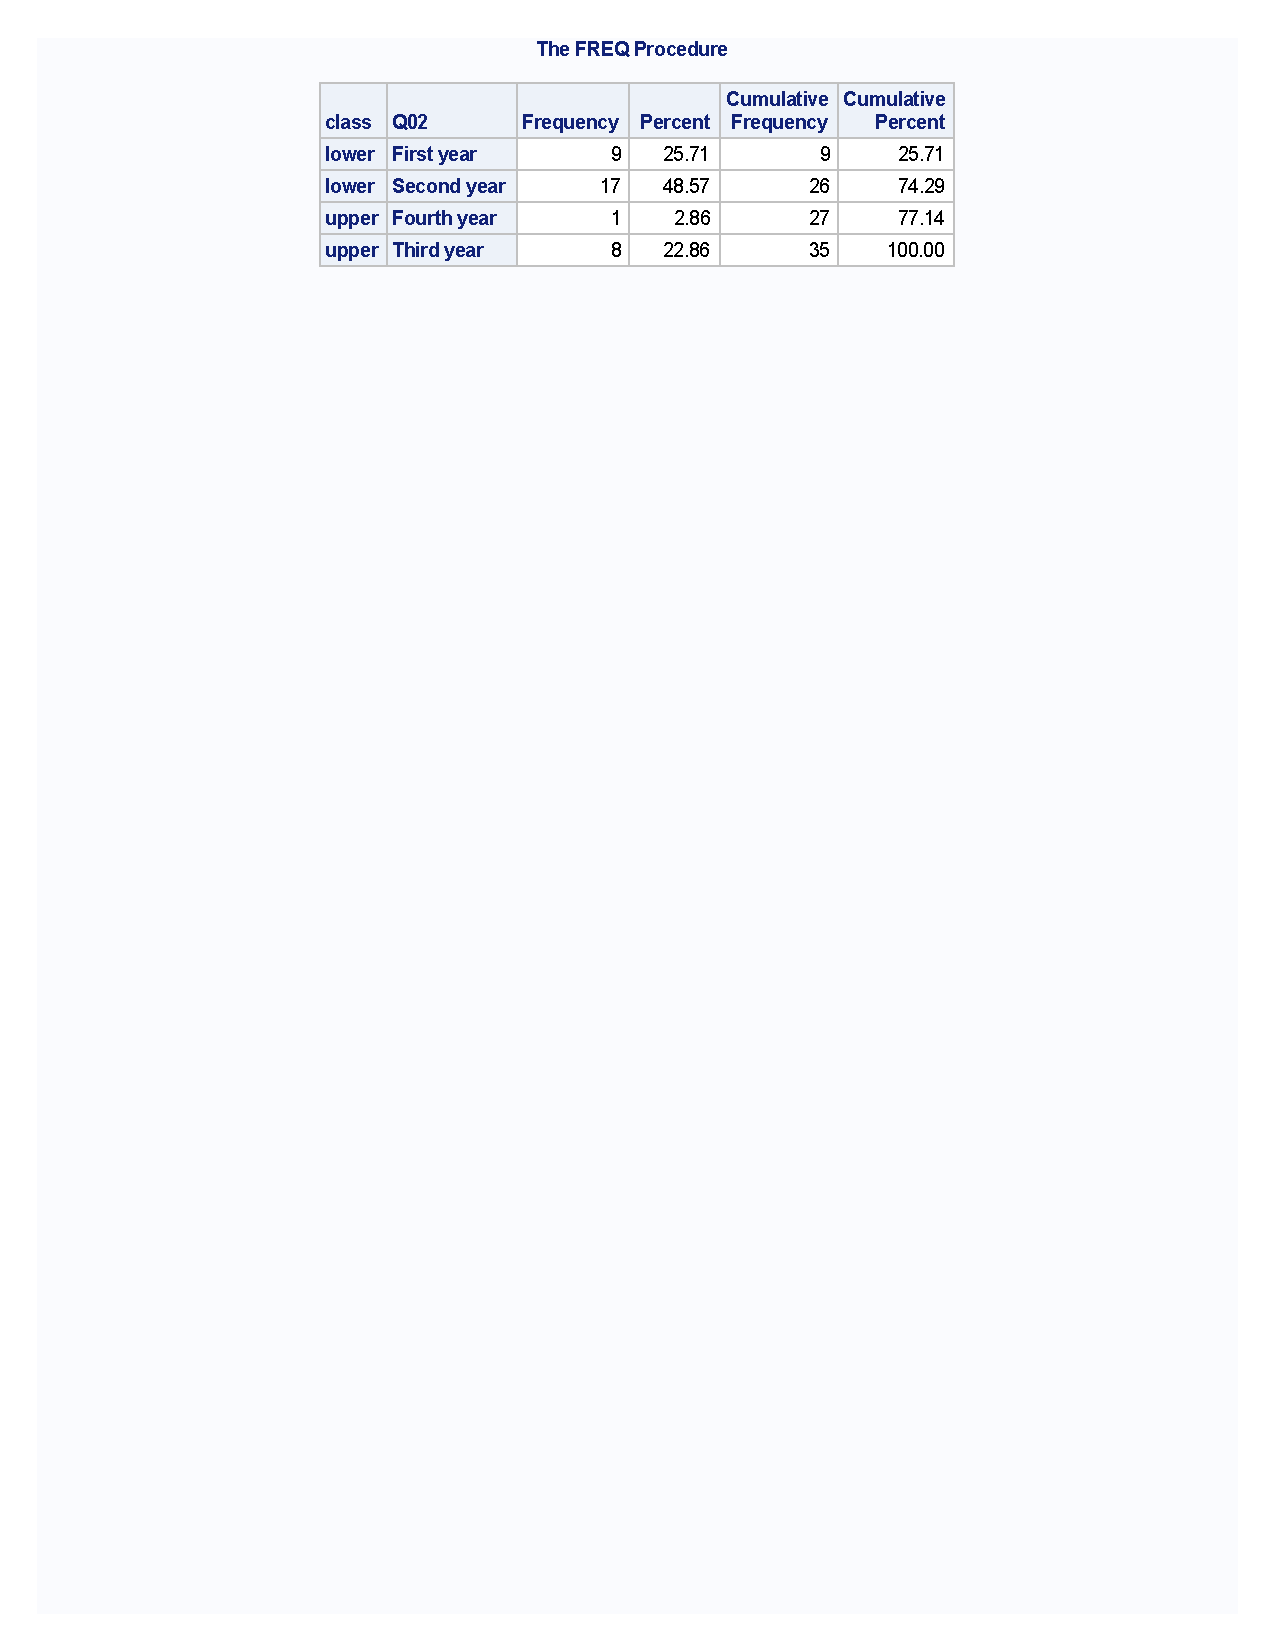
\includegraphics[trim=5cm 22cm 5cm 0.5cm,clip,width=1.0\textwidth]{L9_ccstep3b.pdf}
\emp
\end{frame}

%===========================================================================================================================
\section[Quantitative to Quantitative]{Quantitative to Quantitative}
%===========================================================================================================================
\subsection{}
\begin{frame}
\tableofcontents[currentsection, hideallsubsections]
\end{frame}

\begin{frame}[fragile]
\ft{Step 1: Get to know your data.}
\framesubtitle{\underline{Lab 4 Q6:} Create a new variable called \texttt{GPA\_clean} that is a copy of the GPA variable.  Re-code the unusual values that you identified in the previous question to missing. }
\begin{enumerate}[a.]
\item Identify existing values and/or unusual values
\item Identify if missing values are present
\item Identify how many observations had the unusual values
\item Identify which observations had the unusual values
\end{enumerate}
\vskip10pt
\bmp{1.0\textwidth}
\footnotesize
\begin{code}{.0}
PROC MEANS DATA = work.survey2 VAR  Q04; RUN;

PROC UNIVARIATE DATA = work.survey2; VAR Q04; RUN;

PROC FREQ DATA = work.survey2; TABLES Q04; RUN;

PROC PRINT DATA = work.survey2; WHERE Q04 > 4; RUN;
\end{code}
\emp
\end{frame}


\begin{frame}[fragile]
\ft{Step 2: Create clean new variables with desired result.}
\framesubtitle{\underline{Lab 4 Q6:} Create a new variable called \texttt{GPA\_clean} that is a copy of the GPA variable.  Re-code the unusual values that you identified in the previous question to missing. }
\bmp{1.0\textwidth}
\footnotesize
\begin{code}{.0}
GPA_clean = Q04 ;
IF GPA_clean > 4 THEN GPA_clean = . ;
\end{code}
\emp
\end{frame}

\begin{frame}[fragile]
\ft{Step 3: Verify that coding was done correctly.}
\framesubtitle{\underline{Lab 4 Q6:} Create a new variable called \texttt{GPA\_clean} that is a copy of the GPA variable.  Re-code the unusual values that you identified in the previous question to missing. }
\bmp{0.5\textwidth}
\footnotesize
\begin{code}{.0}
PROC MEANS DATA = survey3 ;
	VAR Q04 GPA_clean ;
RUN ;
\end{code}
\emp
\bmp{0.02\textwidth} \hspace{1in} \emp
\bmp{0.5\textwidth}
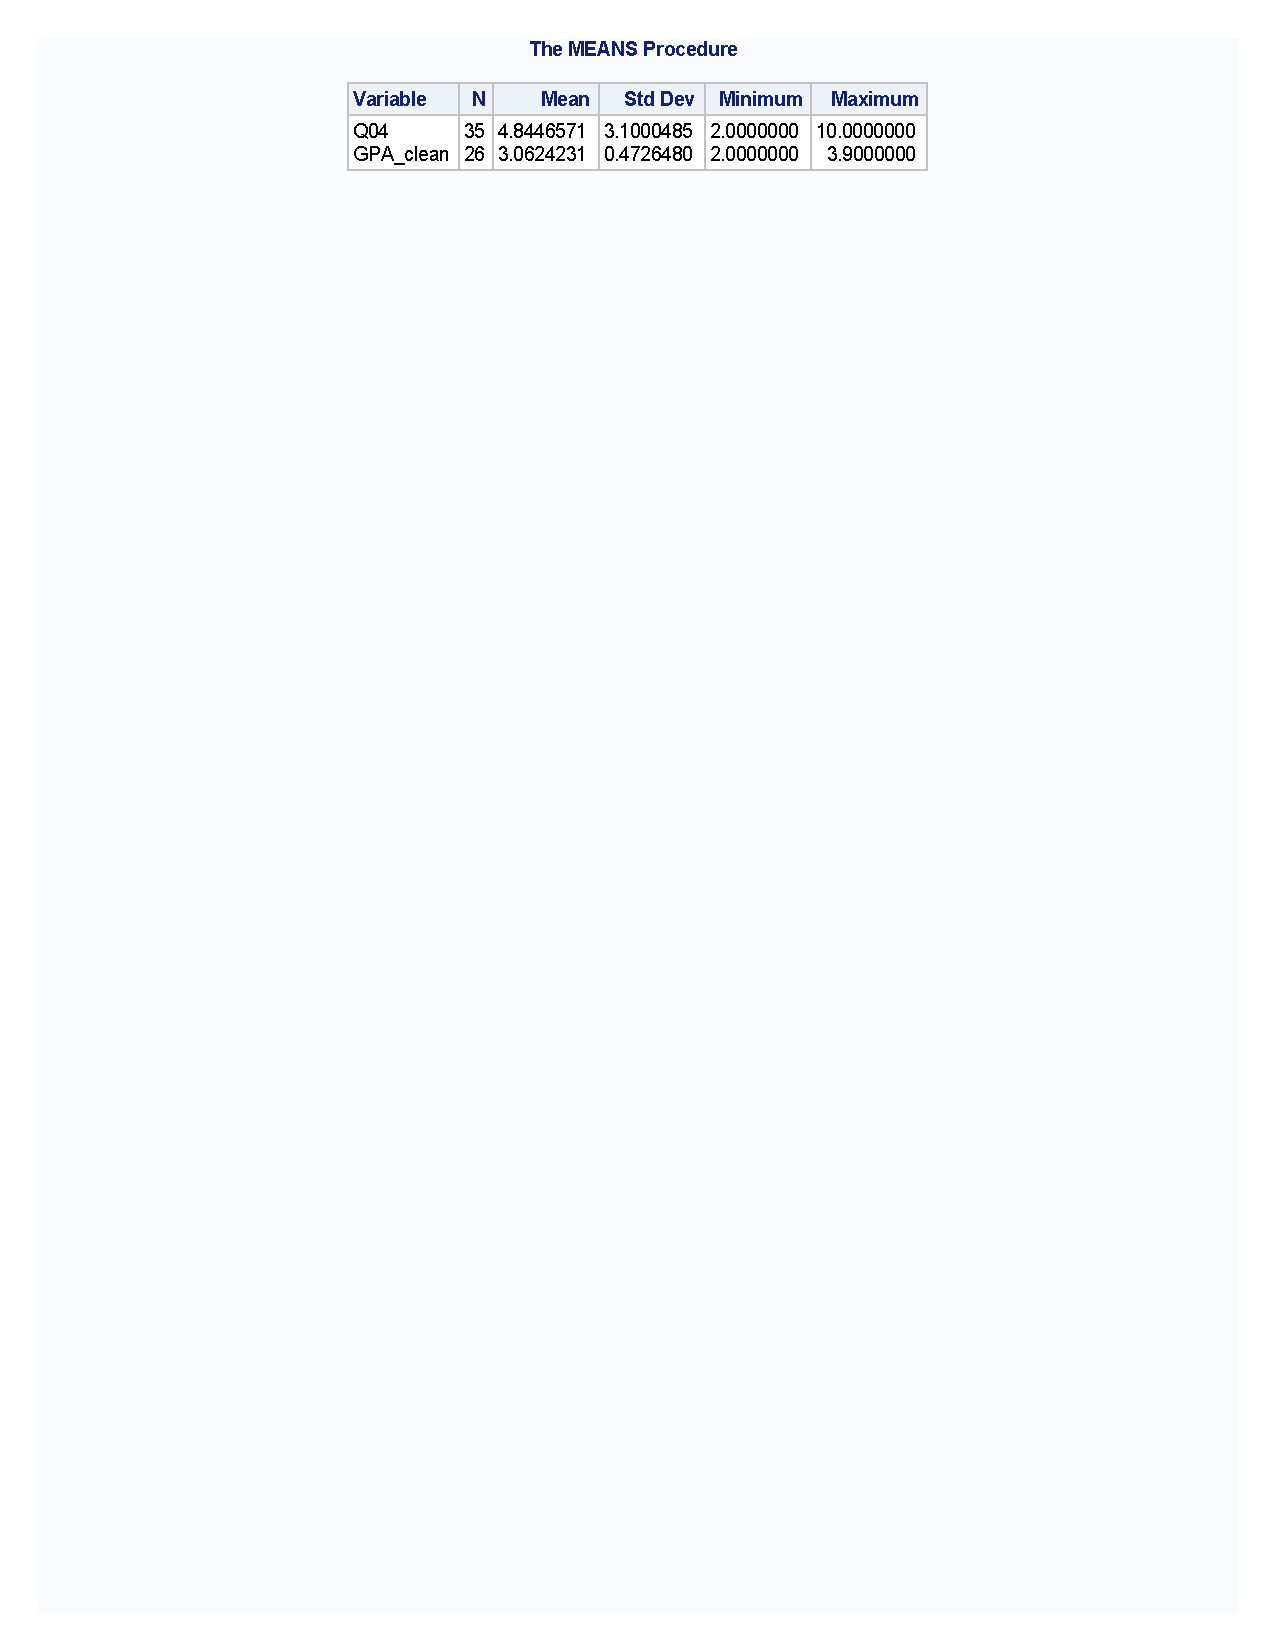
\includegraphics[trim=5cm 24cm 5cm 0.5cm,clip,width=1.0\textwidth]{L9_qqstep3a.pdf}
\emp
\end{frame}

\begin{frame}[fragile]
\ft{Step 3: Verify that coding was done correctly, better.}
\framesubtitle{\underline{Lab 4 Q6:} Create a new variable called \texttt{GPA\_clean} that is a copy of the GPA variable.  Re-code the unusual values that you identified in the previous question to missing. }
\bmp{0.5\textwidth}
\footnotesize
\begin{code}{.0}
PROC FREQ DATA = survey3 ;
   TABLES Q04 * GPA_clean /
   LIST MISSING ;
RUN ;
\end{code}
\emp
\bmp{0.02\textwidth} \hspace{1in} \emp
\bmp{0.5\textwidth}
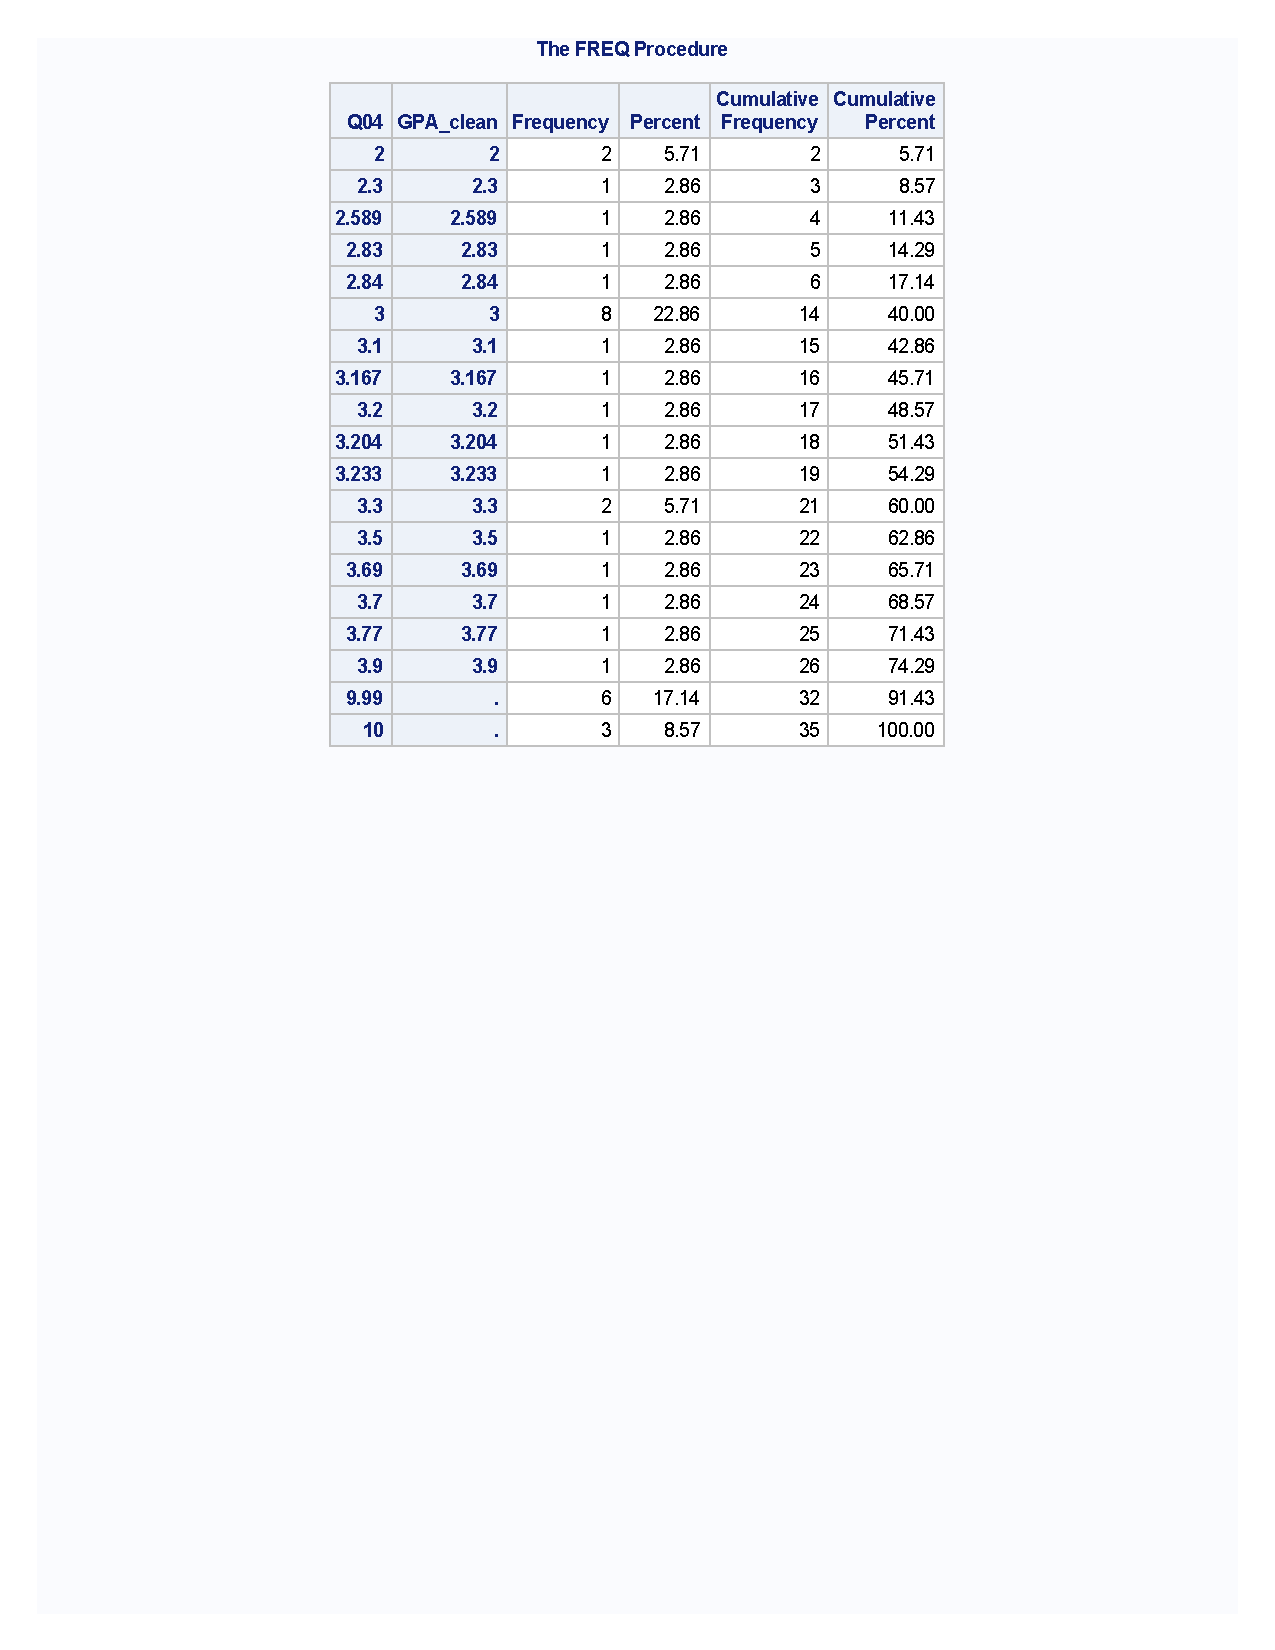
\includegraphics[trim=5cm 15cm 5cm 0.5cm,clip,width=1.0\textwidth]{L9_qqstep3b.pdf}
\emp
\end{frame}


%===========================================================================================================================
\section[Quantitative to Categorical]{Quantitative to Categorical}
%===========================================================================================================================
\subsection{}
\begin{frame}
\tableofcontents[currentsection, hideallsubsections]
\end{frame}

\begin{frame}[fragile]
\ft{Step 1: Get to know your data.}
\framesubtitle{\underline{Lab 4 Q13:} Use the \texttt{GPA\_clean} variable to create a new variable called \texttt{honors} that classifies students according to their current GPA; students who do not yet achieve honors should be classified as ``none''.}
\begin{enumerate}[a.]
\item Identify existing values and/or unusual values
\item Identify if missing values are present
\item Identify how many observations had the unusual values
\item Identify which observations had the unusual values
\end{enumerate}
\vskip10pt
\bmp{1.0\textwidth}
\footnotesize
\begin{code}{.0}
PROC MEANS DATA = work.survey3; VAR GPA_clean; RUN;

PROC UNIVARIATE DATA = work.survey3; VAR GPA_clean; RUN;

PROC FREQ DATA = work.survey3; TABLES GPA_clean; RUN;

PROC PRINT DATA = work.survey3; WHERE GPA_clean = . ; RUN;
\end{code}
\emp
\end{frame}


\begin{frame}[fragile]
\ft{Step 2: Create clean new variables with desired result, method 1.}
\framesubtitle{\underline{Lab 4 Q13:} Use the \texttt{GPA\_clean} variable to create a new variable called \texttt{honors} that classifies students according to their current GPA; students who do not yet achieve honors should be classified as ``none''.}
\bmp{1.06\textwidth}
\footnotesize
\begin{code}{.0}
LENGTH honors $ 20 ;
IF GPA_clean = . THEN honors = "" ;
ELSE IF GPA_clean >= 3.85 THEN honors = "Summa cum laude" ;
ELSE IF 3.70 <= GPA_clean < 3.85 THEN honors = "Magna cum laude" ;
ELSE IF 3.50 <= GPA_clean < 3.70 THEN honors = "Cum laude" ;
ELSE honors = "none" ;
\end{code}
\emp
\end{frame}

\begin{frame}[fragile]
\ft{Step 3: Verify that coding was done correctly, method 1.}
\framesubtitle{\underline{Lab 4 Q13:} Use the \texttt{GPA\_clean} variable to create a new variable called \texttt{honors} that classifies students according to their current GPA; students who do not yet achieve honors should be classified as ``none''.}\bmp{0.5\textwidth}
\footnotesize
\begin{code}{.0}
PROC MEANS DATA = survey4 ;
   VAR GPA_clean ;
   CLASS honors ;
RUN ;
\end{code}
\emp
\bmp{0.02\textwidth} \hspace{1in} \emp
\bmp{0.5\textwidth}
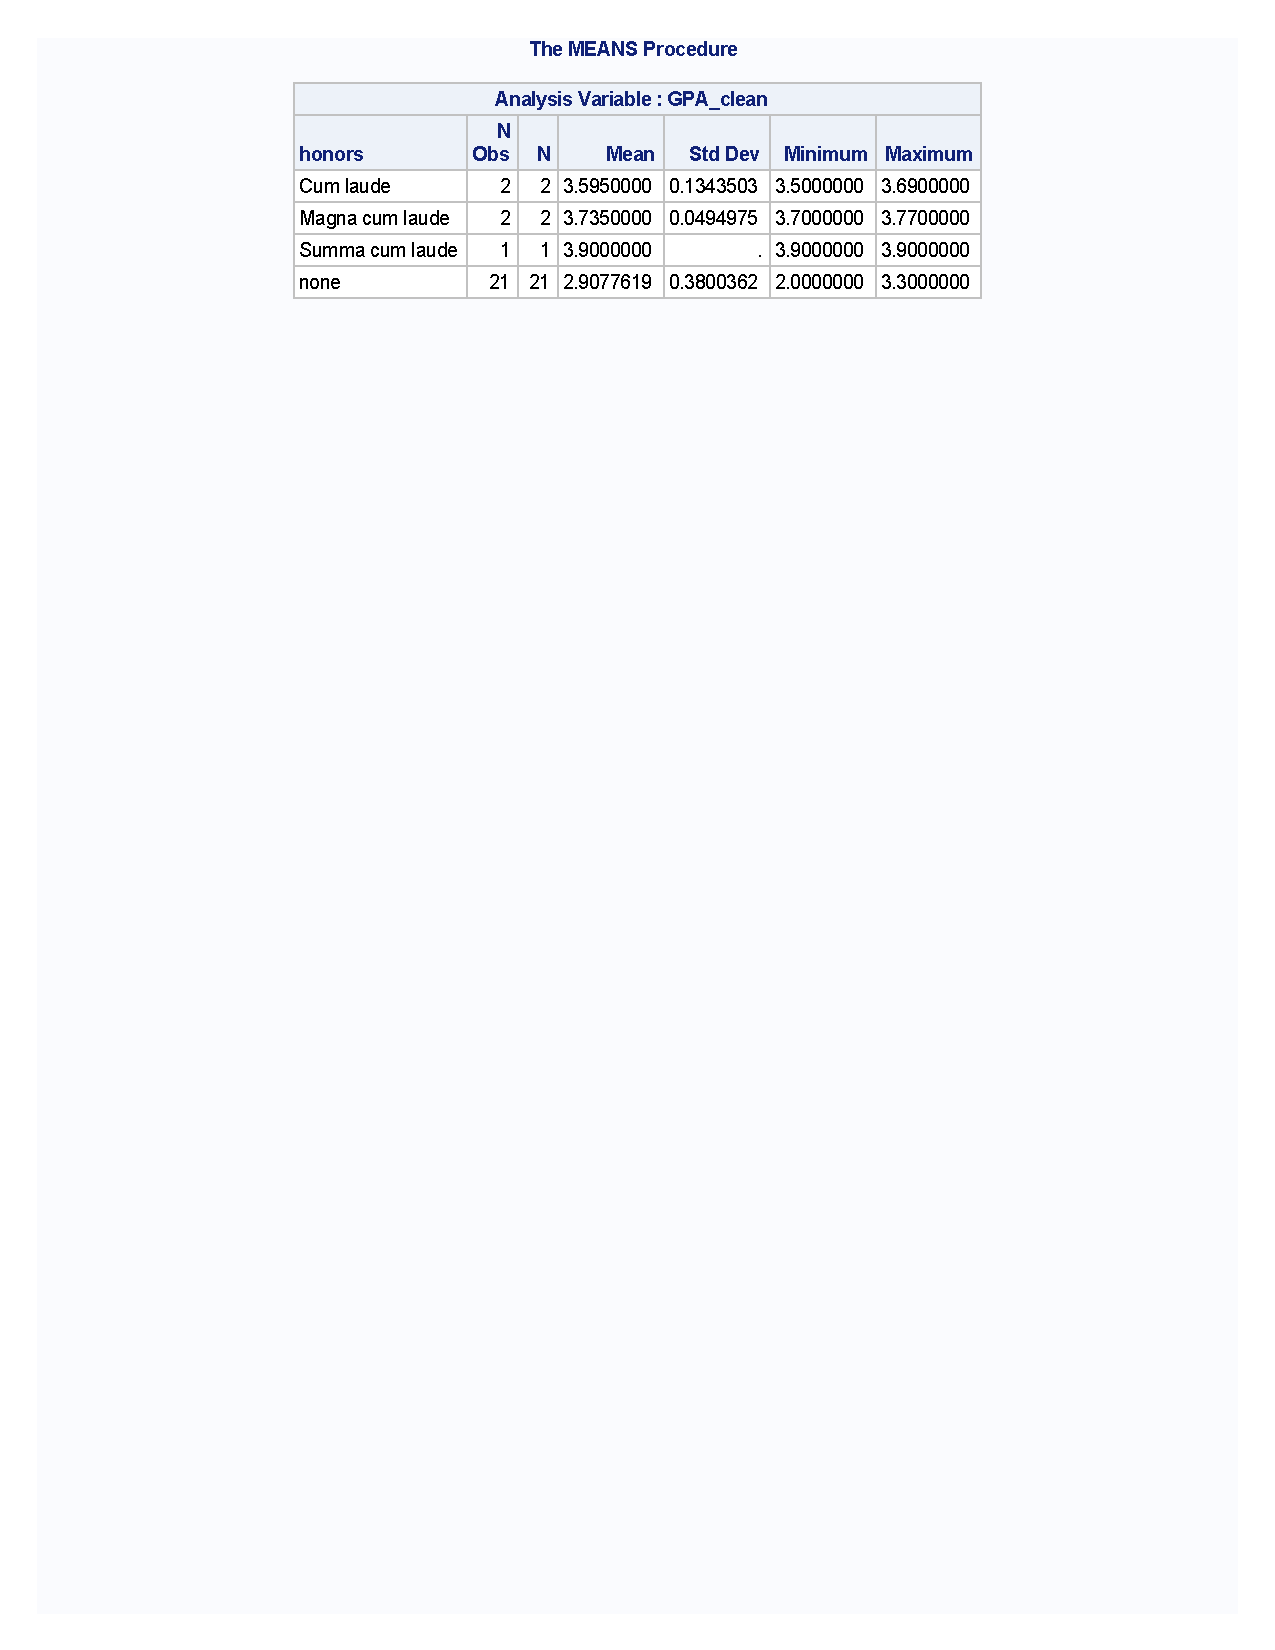
\includegraphics[trim=4cm 22cm 4cm 0.5cm,clip,width=1.0\textwidth]{L9_qcstep3a.pdf}
\emp
\end{frame}

\begin{frame}[fragile]
\ft{Step 3: Verify that coding was done correctly, method 2.}
\framesubtitle{\underline{Lab 4 Q13:} Use the \texttt{GPA\_clean} variable to create a new variable called \texttt{honors} that classifies students according to their current GPA; students who do not yet achieve honors should be classified as ``none''.}
\bmp{0.5\textwidth}
\footnotesize
\begin{code}{.0}
PROC FREQ DATA = survey4 ;
  TABLES honors * GPA_clean /
  LIST MISSING;
RUN ;
\end{code}
\emp
\bmp{0.02\textwidth} \hspace{1in} \emp
\bmp{0.5\textwidth}
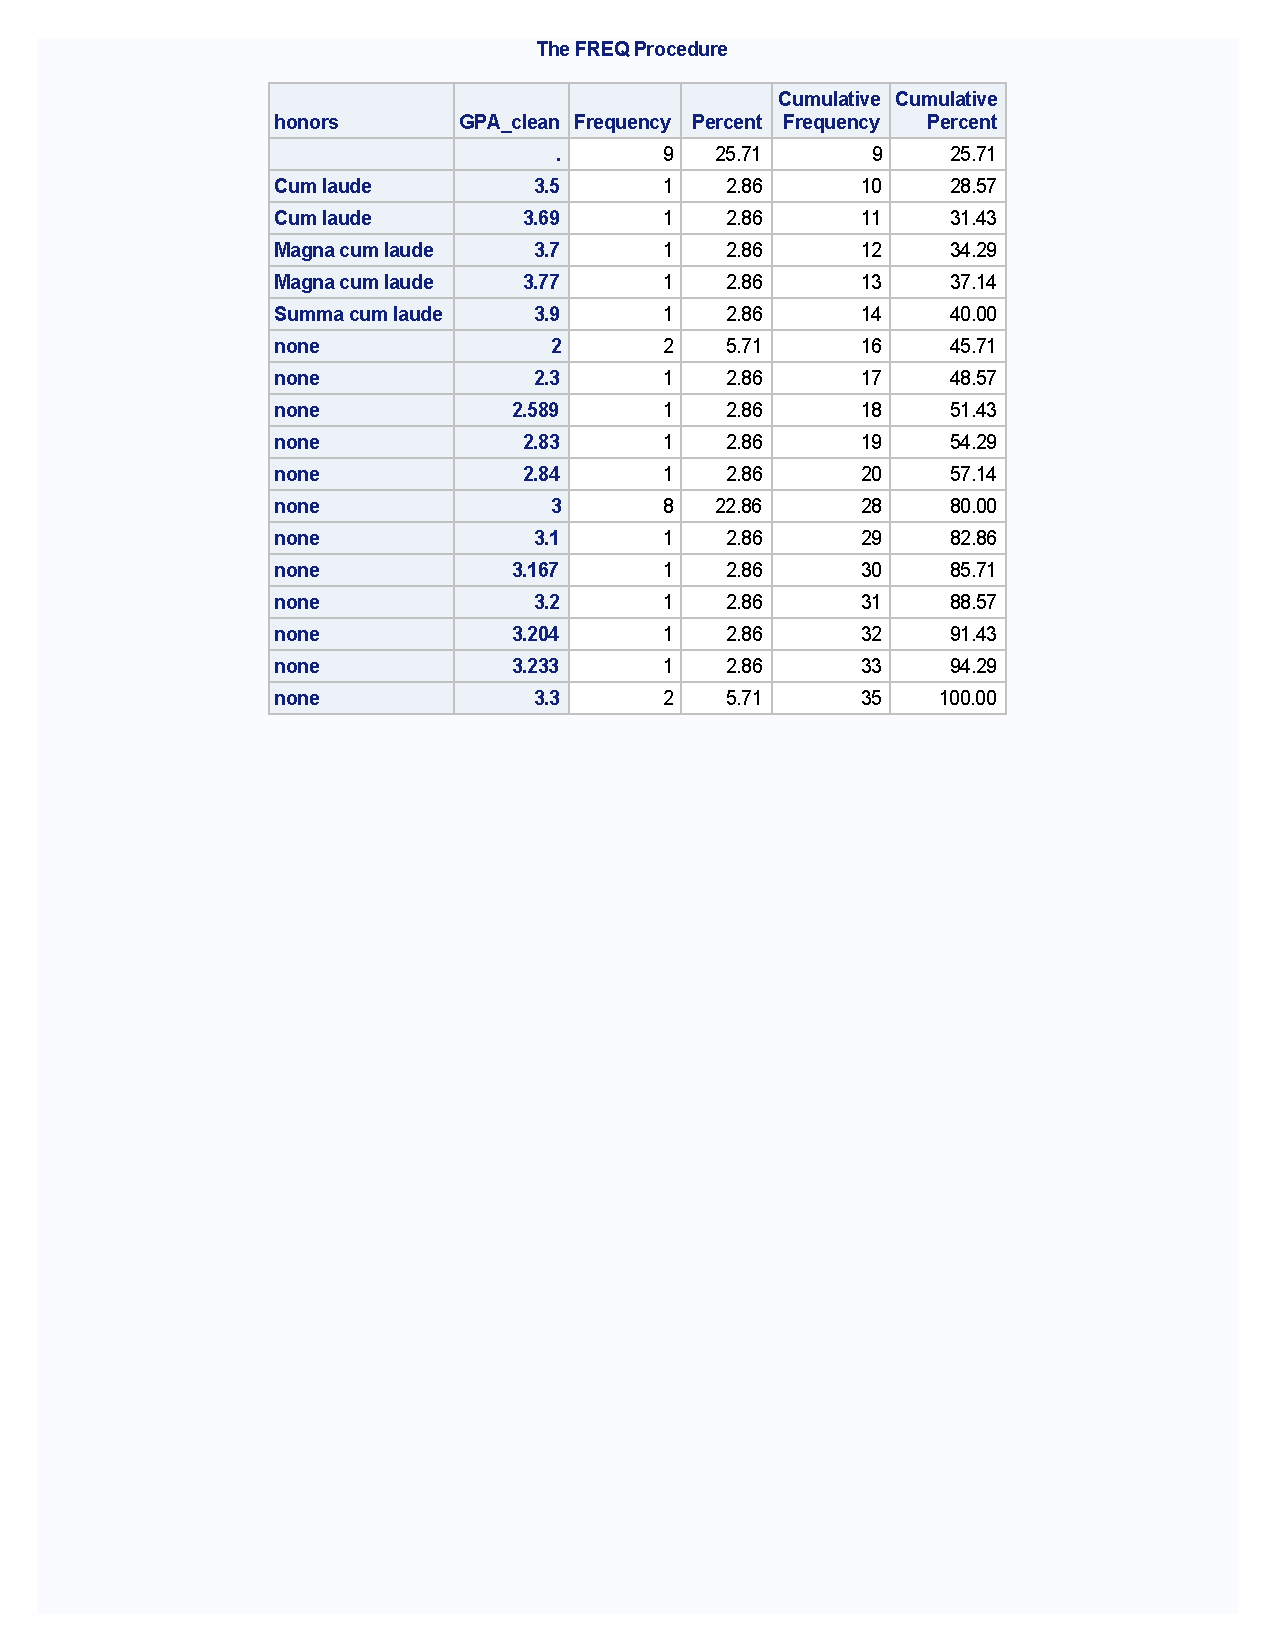
\includegraphics[trim=3cm 15cm 3cm 0.5cm,clip,width=1.0\textwidth]{L9_qcstep3b.pdf}
\emp
\end{frame}

\end{document} 